\documentclass[10pt]{article}
\usepackage[margin=24mm]{geometry}
\usepackage{fontspec}
\usepackage{unicode-math}
\usepackage{amsmath,booktabs,graphicx,xurl}
\usepackage{microtype}
\usepackage{hyperref}
\hypersetup{colorlinks=true,linkcolor=blue,citecolor=blue,urlcolor=blue}
\setlength{\parskip}{0.45em}
\setlength{\parindent}{0pt}
\setlength{\emergencystretch}{3em}
\newcommand{\doctype}{Preprint}
\newcommand{\docversion}{v1.0}
\newcommand{\docdate}{31 October 2026}
\newcommand{\versiondoi}{10.5281/zenodo.23833135}
\newcommand{\conceptdoi}{10.5281/zenodo.23833134}
\newcommand{\docrepo}{https://github.com/fsantibanezleal/CAOS\_OreFlow}
\newcommand{\headerblock}{%
\begin{center}
\fbox{\parbox{0.94\textwidth}{\small\raggedright
\textbf{\doctype} \quad$\cdot$\quad \docversion, \docdate \quad$\cdot$\quad Licence CC BY 4.0\\[2pt]
CAOS open-research programme \quad$\cdot$\quad mineral-processing optimization\\[2pt]
Version DOI \href{https://doi.org/\versiondoi}{\texttt{\versiondoi}} \quad$\cdot$\quad
concept DOI (always latest) \href{https://doi.org/\conceptdoi}{\texttt{\conceptdoi}}\\[2pt]
Not peer reviewed. Source code, data and computational records: \href{https://github.com/fsantibanezleal/CAOS_OreFlow}{\texttt{github.com/fsantibanezleal/CAOS\_OreFlow}}
}}
\end{center}
\vspace{4pt}}
\title{When a screened pattern search spends more simulator calls: evidence from mineral-processing circuit cases}
\author{Felipe Santibáñez-Leal, ORCID 0000-0002-0150-3246}
\date{}
\begin{document}
\maketitle
\headerblock

\section*{Abstract}
Surrogate models can reduce the cost of optimizing computationally expensive process simulators, but their value depends on whether screening eliminates enough exact evaluations to offset the evaluations it adds and whether it changes the selected operating decision. We compare a Gaussian-process-screened generalized pattern search with the same progressive-barrier search without screening. Both procedures use the same starts, bounds, objective weights and exact circuit evaluator. In 72 target-mode variants spanning twelve authored mineral-processing cases, the screened procedure used 26,367 exact engine evaluations, compared with 22,487 without screening, a 17.25\% increase. It used more evaluations in 68 variants, the same number in four and fewer in none. Both procedures returned feasible optima in 70 variants and infeasibility in two; their terminal outcomes matched in 65. In the seven remaining feasible comparisons, absolute differences in recovered primary metal did not exceed 0.0027 t/h (0.017\%). Across 5,811 surrogate-selected proposals, 901 improved the incumbent. Absolute recovery-prediction error had a mean of 0.71 percentage points, a median of 0.48 points and a maximum of 38.16 points. The screen therefore preserved outcomes closely on this authored suite but did not reduce simulator cost. The results do not establish performance on plant-calibrated circuits.

\section{Introduction}
Grinding, classification and flotation decisions interact through nonlinear balances, equipment limits and product-quality constraints. Direct simulation can be expensive when an optimizer repeatedly evaluates a complete flowsheet. A learned approximation may reduce that cost by ranking candidates before exact simulation, but only if the number of avoided simulator calls exceeds the number of additional calls caused by the screening rule. Prediction accuracy alone is insufficient: optimization depends on errors near competing candidates and on the geometry of the feasible region.

Surrogate models have been used to approximate phenomenological comminution circuits. Koh et al. report a neural-network surrogate for simulator throughput with substantial speedup on their studied circuit and data design \cite{Koh2021}. More generally, surrogate management methods combine approximate models with exact evaluations and retain convergence safeguards for the original problem \cite{Booker1999}. Generalized pattern search provides derivative-free search with convergence results under specified smoothness and direction-set assumptions \cite{Torczon1997,AudetDennis2006}. These results motivate guarded screening, but do not imply that a particular screen reduces calls or preserves a particular finite-budget solution.

This study evaluates one integrated procedure on OreFlow's committed case records. It asks two bounded questions: does screening reduce exact engine evaluations, and how closely do the screened and unscreened searches agree on feasibility and recovered metal? The cases are authored scenarios rather than measured operating data. The result is therefore an algorithmic comparison within a declared simulator domain, not a plant-performance claim.

\section{Related work}
Koh et al. trained a deep neural model to reproduce a phenomenological comminution-circuit simulator and used the approximation to accelerate scenario evaluation \cite{Koh2021}. That work addresses approximation of simulator outputs. Here, the object of evaluation is the effect of a surrogate-driven search step inside a bounded derivative-free optimizer, including the exact-call cost and terminal decision relative to an unscreened control.

The surrogate management framework formalizes the interplay between approximation models and exact objective evaluations \cite{Booker1999}. Generalized pattern search methods offer convergence properties for suitable objective functions and generating directions; those properties do not automatically transfer to a modified search step without the relevant assumptions and proof \cite{Torczon1997,AudetDennis2006}. Accordingly, this experiment reports finite-suite behavior and makes no global-convergence claim for the screened implementation.

\section{Method}
\subsection{Process decision problem}
For each case, the search varies the grind target, collector dose and rougher gas velocity within the case contract. The evaluator returns recovered primary metal $M$ in t/h, recovery, concentrate grade, total specific energy $E$ in kWh/t, power and water use. For a selected recovery weight $w\in[0,1]$, the normalized objective is
\begin{equation}
 J(x;w)=w\frac{M(x)}{M_0}-(1-w)\frac{E(x)}{E_0},
\end{equation}
where $M_0$ and $E_0$ are the values at the variant's base operating point. Grade, installed power and water limits are treated as relaxable constraints through a progressive barrier; contract bounds on decisions are unrelaxable. The recorded weight path, starts and stopping rules are identical between paired searches.

\subsection{Exact and screened searches}
The baseline is a generalized pattern search with a progressive feasibility barrier. The screened procedure uses the same engine, objective, starts, mesh, bounds, constraints and stopping budget. At each iteration, a Gaussian-process recovery model and the exported learned evaluator score candidate points one and two mesh steps from feasible and infeasible incumbents. A proposal is eligible only when the learned-state guard passes and the Gaussian-process 95\% recovery half-width does not exceed five percentage points. The highest predicted objective among eligible points is evaluated by the exact circuit engine. Only that engine result can update the incumbent or become a reported optimum. If no candidate passes, the search performs its ordinary polling step.

Each case record contains screen counts, accepted proposals, the surrogate and engine results for each proposal, the evaluation count, the terminal outcome and a paired unscreened search from the same starts. This paired design isolates the computational effect of the screen within the simulator and its finite search settings. It does not estimate runtime on a plant control system.

\subsection{Evaluation set and measures}
The baked suite contains 96 variants: 72 target-mode variants and 24 classifier-cut variants. The latter are intentionally unscreened because the learned screen's features do not cover that circuit mode. Two target-mode iron-magnetite variants have no feasible solution under their declared constraints. We therefore report the paired evaluation cost over all 72 target-mode records and compare optimum decisions only for the 70 records where both searches return a feasible optimum. A matching infeasible result in both procedures counts as a matching terminal outcome, not as an optimum.

The primary cost measure is the ratio of total exact engine evaluations. Secondary measures are per-variant cost ordering, terminal-outcome agreement, recovered-metal difference, number of proposals that improve the incumbent and absolute recovery error at proposed points. Percentage-point errors are differences between recovery percentages, not relative percentage errors.

\section{Results}
\subsection{Exact evaluation cost}
Across the 72 paired target-mode variants, screening used 26,367 engine evaluations; the baseline used 22,487. The relative increase is
\begin{equation}
100\left(\frac{26{,}367}{22{,}487}-1\right)=17.25\%.
\end{equation}
Screening cost more in 68 variants and tied in four; it saved evaluations in none. The comparison includes the entire recorded weight path and all starts for each variant. It is not a wall-clock benchmark, and it excludes the one-time training and export cost of the surrogate.

\begin{figure}[ht]
\centering
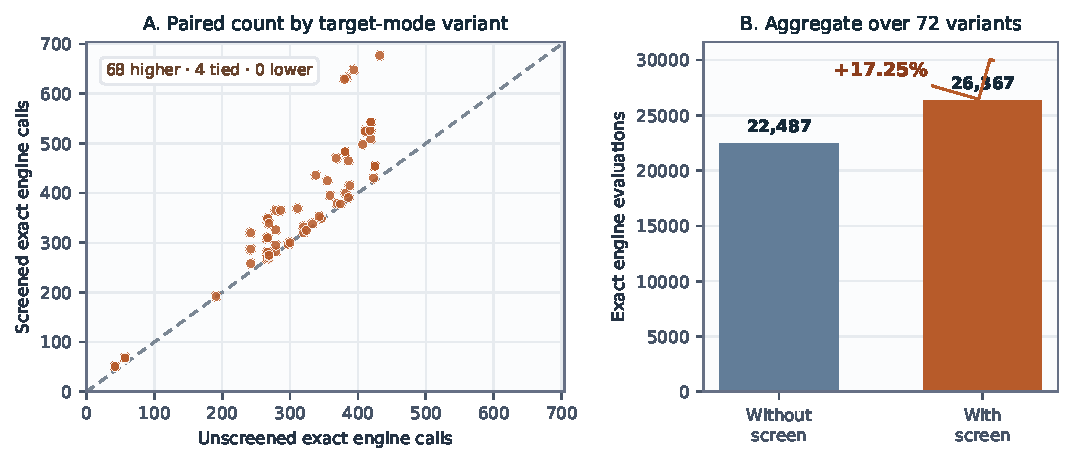
\includegraphics[width=0.98\textwidth]{figure-results.pdf}
\caption{Paired exact-engine calls for the 72 target-mode variants. Points above the identity line require more calls with screening. The aggregate panel compares the sums over the same paired records.}
\label{fig:cost}
\end{figure}

\begin{table}[ht]
\centering
\caption{Paired optimization results on the 72 target-mode variants.}
\label{tab:paired}
\begin{tabular}{lr}
\toprule
Measure & Result \\
\midrule
Authored cases & 12 \\
Target-mode variants & 72 \\
Feasible optima in both searches & 70 \\
Infeasible outcomes in both searches & 2 \\
Exact engine evaluations, screened & 26,367 \\
Exact engine evaluations, unscreened & 22,487 \\
Cost change & +17.25\% \\
More / tied / fewer evaluations & 68 / 4 / 0 \\
Same terminal outcome & 65 / 72 \\
\bottomrule
\end{tabular}
\end{table}

\subsection{Decision agreement}
Both procedures return feasible optima in 70 variants and classify the remaining two as infeasible. They return the same terminal outcome in 65 of 72 variants: the 63 exactly matching feasible decision vectors plus the two matching infeasible outcomes. Seven feasible variants select different decision vectors. Across those seven, the largest absolute difference in recovered primary metal is 0.002653 t/h, or 0.0168\% relative to the larger value. Five favor the unscreened result in recovered metal and two favor the screened result. This close numerical agreement on these cases does not show that screening is safe for other inputs, constraints or stopping budgets.

\subsection{Proposal behavior and prediction errors}
The screened search records 79,035 candidate evaluations by the screening logic. Nineteen are rejected by the learned-state guard and 48,266 by the uncertainty-width rule. The algorithm sends 5,811 selected proposals to the engine; 901, or 15.5\%, improve the incumbent. For those proposals, the mean absolute recovery error is 0.712 percentage points, the median is 0.483 points and the maximum is 38.158 points. The large maximum is material: the confidence-width filter did not eliminate every large pointwise error in the proposal record. The evidence does not support describing the surrogate as uniformly accurate where it is used.

\section{Discussion}
For this suite, screening yields a striking separation between decision agreement and computational efficiency. The selected decisions are usually identical and the measured metal differences are small, yet the screened search evaluates the circuit more often. This is consistent with a mechanism in which the screen adds exact evaluations at selected candidates without removing enough ordinary polling evaluations. Close final decisions do not compensate for a 17.25\% increase in the measured call count when the objective of screening is to reduce simulator work.

The result also illustrates why average prediction error is not a sufficient screen diagnostic. Optimization depends on candidate ranking near the incumbent, uncertainty calibration in the feasible region and how many candidates the screen makes the exact evaluator inspect. The observed maximum recovery error of 38.16 percentage points cautions against treating a nominal confidence-width threshold as a universal safety guarantee. Independent calibration on the exact region of use and a prospective test on new cases would be needed before relying on the screen outside this authored suite.

The comparator is deliberately narrow: the same multistart generalized pattern search with screening switched off. The experiment does not compare global optimization methods, alternative surrogate-management strategies or wall-clock performance on a calibrated plant model. Evaluation counts include the recorded four-weight path and do not include surrogate fitting time. The case suite uses authored inputs and simulator-generated values, so it cannot establish transfer to unseen plants or ores.

\section{Limitations}
All optimization outcomes are generated by an authored, steady-state process simulator. They are not measurements from operating plants. Model-form error, changing ore, plant instrumentation error, control-system latency and economic uncertainty are outside this experiment. The finite set of twelve cases does not represent the full mineral-processing design space.

The paired searches share a finite starting set, mesh and evaluation budget. Agreement is conditional on those choices and does not establish global optimality. The progressive-barrier method has established convergence analyses under their stated assumptions; this implementation's surrogate-selected search modification is not accompanied by a new convergence proof. The call-count measure also omits time spent fitting, loading and evaluating the surrogate, as well as parallel execution effects.

\section{Conclusions}
The guarded Gaussian-process screen did not reduce exact circuit-engine evaluations on OreFlow's 72 target-mode optimization records. It used 17.25\% more calls than the paired unscreened procedure, saved calls in no variant and produced terminal outcomes matching in 65 cases. Seven feasible optima differed, with at most 0.002653 t/h difference in recovered primary metal. The maximum observed proposal recovery error was 38.16 percentage points despite the uncertainty-width filter. These findings support retaining the screen as a reproducible comparison method while rejecting its use as a demonstrated compute-saving accelerator on this suite. A future evaluation would require a new, predeclared screening design, calibration checks on candidate regions and validation on cases not used to design the rule.

\section*{Data and code availability}
The case-level optimization records are committed under \url{https://github.com/fsantibanezleal/CAOS_OreFlow/tree/main/data/derived/cases}; the implementation and tests are in the same public repository. Each record stores paired search counts, proposals, engine outcomes and terminal decisions. The records are simulator outputs from authored scenarios and are not plant data.

\begin{thebibliography}{9}
\bibitem{AudetDennis2006} C. Audet and J. E. Dennis, Jr., ``Mesh adaptive direct search algorithms for constrained optimization,'' \emph{SIAM Journal on Optimization}, vol. 17, no. 1, pp. 188--217, 2006. doi: \href{https://doi.org/10.1137/040603371}{10.1137/040603371}.
\bibitem{Booker1999} A. J. Booker, J. E. Dennis, Jr., P. D. Frank, D. B. Serafini, V. Torczon, and M. W. Trosset, ``A rigorous framework for optimization of expensive functions by surrogates,'' \emph{Structural Optimization}, vol. 17, pp. 1--13, 1999. doi: \href{https://doi.org/10.1007/BF01197708}{10.1007/BF01197708}.
\bibitem{Koh2021} E. J. Y. Koh, E. Amini, G. J. McLachlan, and N. Beaton, ``Utilising a deep neural network as a surrogate model to approximate phenomenological models of a comminution circuit for faster simulations,'' \emph{Minerals Engineering}, vol. 170, article 107026, 2021. doi: \href{https://doi.org/10.1016/j.mineng.2021.107026}{10.1016/j.mineng.2021.107026}.
\bibitem{Torczon1997} V. Torczon, ``On the convergence of pattern search algorithms,'' \emph{SIAM Journal on Optimization}, vol. 7, no. 1, pp. 1--25, 1997. doi: \href{https://doi.org/10.1137/S1052623493250780}{10.1137/S1052623493250780}.
\end{thebibliography}
\end{document}

